\subsection{Time Constant Effect on Beam and Pointing}

\paragraph{Description:}
The time constants can both shift the detector pointing and smear the beam, resulting in an increase in the measured beam width. To estimate these effects the beam can be approximated as a Gaussian with a full width at half maximum of $FWHM$. The experiment is assumed to scan at a rate of $f_{scan}$ at an elevation $\theta_{el}$. The scanning speed on the sky $f_{sky}$ is then given by $f_{sky}=f_{scan}\cos{(\theta_{el})}$. The time domain Gaussian beam $\beta (t)$ is then defined as
\begin{equation}
\beta (t)=e^{\frac{-t^2}{2\sigma^2}},
\end{equation}
where $t$ is time and 
\begin{equation}
\sigma=\frac{FWHM}{2f_{sky}\sqrt{2\ln2}}.
\end{equation}
Fourier transforming into frequency space, the beam is given by 
\begin{equation}
\beta (f)=e^{-2 \pi^2 f^2 \sigma^2}.
\end{equation}
The time constants of the detectors act as a low pass filter, so the beam is convolved with a low pass filter given by
\begin{equation}\label{eqn:low_pass}
h(f)=\frac{1-if/f_{3dB}}{1+f^2/f_{3dB}^2}
\end{equation}
and then Fourier transformed back into the time domain to determine the impact on the pointing and beam widths. This treatment assumed that the low pass filter in Equation~\ref{eqn:low_pass} is a good approximation in the range of 3dB frequencies expected for the detectors. Figure~\ref{fig:tc_shift} shows the effect from varying 3dB frequencies on the beam for ABS, which had a $FWHM \approx 30$~arcmin and $f_{sky}\approx 0.5$~deg/s. These calculations give the shift and change in beam width for scanning in one direction, but the telescope scans in both directions. If there are an equal number of scans in each direction, the pointing offset averages out, but an odd number of scans could give a pointing offset. Thus the above calculation gives the maximum pointing offset $\Delta p_{max}$. The effect of scanning both ways further broadens the beam because the average measured beam is the sum of two offset beams as illustrated in Figure~\ref{fig:tc_beam_shift}. To account for this, the two beams from scanning in either direction are approximated as two Gaussian beams and a Gaussian is fit to their sum. From this, $\Delta FWHM$ can be calculated~\cite{Simon_Thesis_2016}. 

\begin{figure}[h!]
\centering
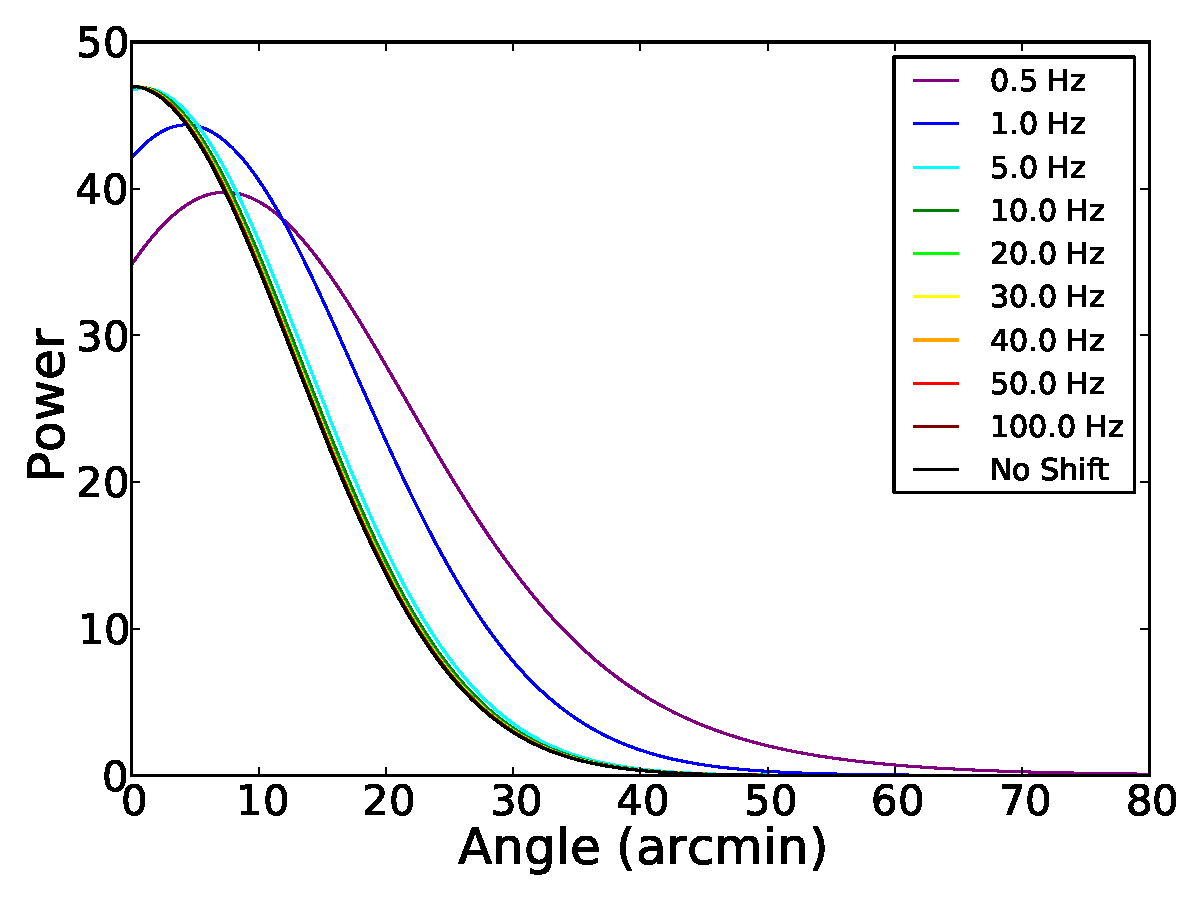
\includegraphics[width=0.90\textwidth]{figures/time_constant_shift.pdf}
\caption{The shift in the pointing and the beam width for an ABS scan in one direction as a result of several time constants is shown above~\cite{Simon_Thesis_2016}. Note that 3dB frequencies above 5~Hz have an extremely small effect. The power is in arbitrary units.}
\label{fig:tc_shift}
\end{figure}


\begin{figure}[h!]
\centering
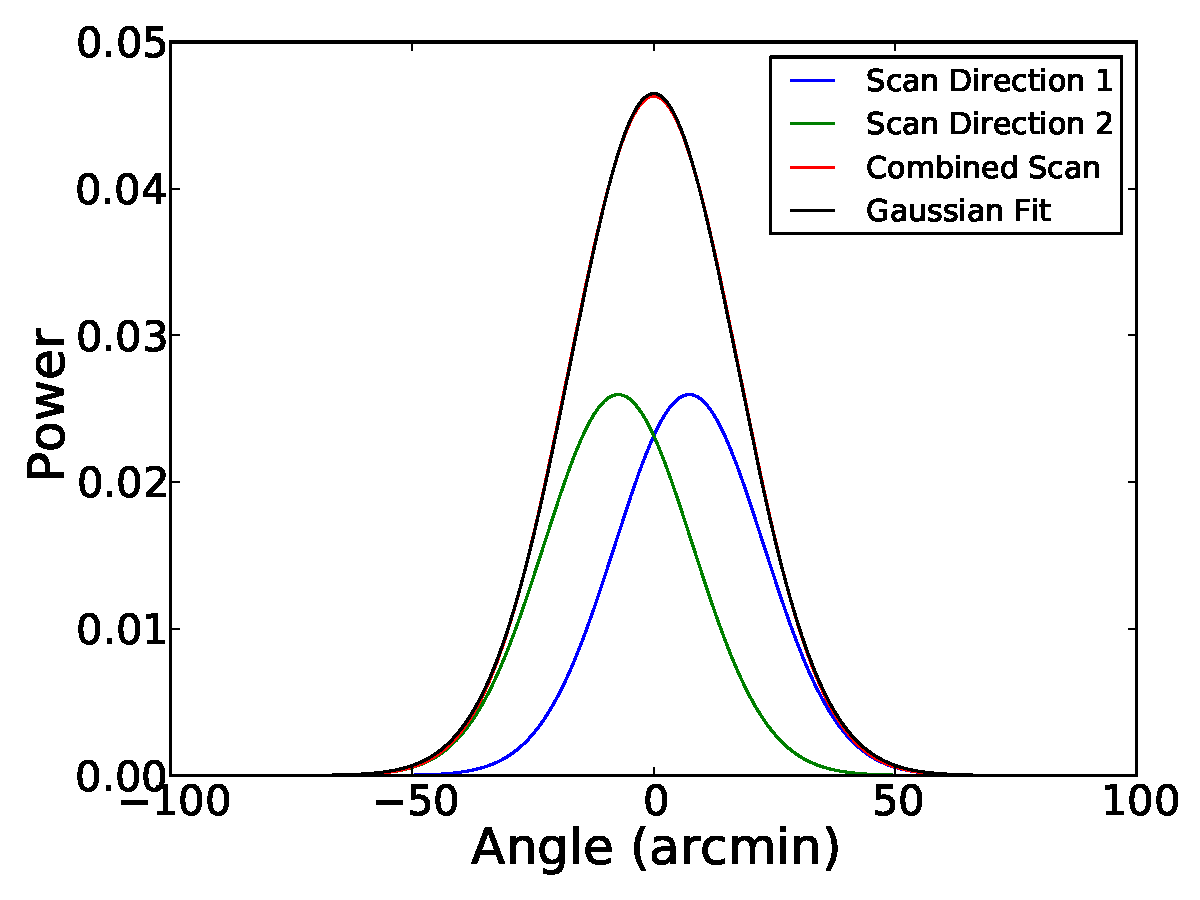
\includegraphics[width=0.80\textwidth]{figures/half_hertz_shift.pdf}
\caption{The shift in the beam width from the time constant when scanning in both directions is estimated with the sum of two Gaussians shifted in pointing and beam width in opposite directions. This can be approximated and fit as a Gaussian. The shift for an extremely slow detector with an $f_{3dB}=0.5$~Hz is shown above for ABS to illustrate this effect~\cite{Simon_Thesis_2016}. The power is in arbitrary units.}
\label{fig:tc_beam_shift}
\end{figure}

\paragraph{Plan to model and/or measure:}

This effect is usually negligible, but it can be approximated as described above quickly and easily given a $f_{3dB}$ value. If the beam is well known, planet scans can be used to determine $\Delta FWHM$ and $\Delta p_{max}$ (though these measurements usually have low signal to noise). A null test split on fast versus slow time constants could help determine if this effect is contaminating the signal, but this null test split is redundant with other time-constant related systematics like the polarization angle rotation.

\paragraph{Uncertainty/Range:}
With the typical $f_{3dB}$ values for CMB experiments, this effect is often negligible, but it is good to check. When modeling this effect, the main uncertainties come from the time constants of the detectors and assuming a purely Gaussian beam. Typically, one can just use the lowest $f_{3dB}$ value expected/measured to put an upper bound on this effect. If the upper bound is negligible, then this effect will be negligible at all higher $f_{3dB}$ values as well. Table~\ref{table:tc_shift} summarizes the impact of the time constants on the ABS beam for various 3dB frequencies.

\begin{table}[h!] 
\begin{center}
  \caption {\textbf{Impact of 3dB Frequency on Beam and Pointing}}\label{table:tc_shift}
\begin{tabular}{|l|l|l|}
  \hline                        
  \textbf{3dB Frequency (Hz)} &  \textbf{Pointing Shift (arcmin)} &  \textbf{$\Delta$ FWHM (arcmin)} \\
  \hline
  0.5 & 7.353 & 10.5 \\
  \hline
  1.0 & 4.313 & 3.7 \\
  \hline
  5.0 & 0.950 & 0.17 \\
 \hline  
  10.0 & 0.477 & 0.043 \\
 \hline  
  20.0 & 0.239 & 0.011 \\
 \hline  
  30.0 & 0.159 & 0.0047 \\
 \hline  
  40.0 & 0.119 & 0.0026 \\
 \hline  
  50.0 & 0.096 & 0.0016 \\
 \hline  
  100.0 & 0.048 & 0.00052 \\
 \hline  
\end{tabular}\\
The pointing shift and beam width changes from different 3dB frequencies are shown above. The typical 3dB frequency of the ABS detectors is $\sim$100~Hz, and the lowest $f_{3dB}$ that passes the data selection criteria is greater than 30~Hz~\cite{Simon_Thesis_2016}.
\end{center}
\end{table}

\paragraph{Parameterization:}
This effect can be parameterized with $\Delta FWHM$ and $\Delta p_{max}$ for a given $f_{3dB}$ value.
